% Program Studi D-IV Komputasi Statistik
% Politeknik Statistika STIS

\documentclass[conference, a4paper]{IEEEtran_ID}
\IEEEoverridecommandlockouts
\usepackage{cite}
\usepackage{fancyhdr}
\usepackage{lastpage}
\usepackage{amsmath,amssymb,amsfonts}
\usepackage{algorithmic}
\usepackage{graphicx}
\usepackage{textcomp}
\usepackage{xcolor}
\usepackage{hyperref}
\def\BibTeX{{\rm B\kern-.05em{\sc i\kern-.025em b}\kern-.08em
    T\kern-.1667em\lower.7ex\hbox{E}\kern-.125emX}}

\pagestyle{fancy}
\fancyhf{}
\lhead{}
\rhead{\footnotesize{Villalobos, E. (2020)}}
\lfoot{}
\rfoot{\thepage { /} \pageref{LastPage}}
\renewcommand{\headrulewidth}{0pt}
\renewcommand{\footrulewidth}{0pt}


\begin{document}

% Elemen judul proposal
\title{\huge{Exploración y visualización de datos, \\ 
y algunas recomendaciones.} % Elemen subjudul proposal
}

% Elemen nama penulis
\author{
\IEEEauthorblockN{\Large{Elena Villalobos Nolasco}}\vspace{0.6em}
\IEEEauthorblockN{Maestría en Ciencia de Datos,}\vspace{0.1em}
\IEEEauthorblockN{Instituto Tecnológico Autónomo de México, ITAM}
}

\maketitle
\thispagestyle{fancy}

%% Elemen ringkasan proposal
%\begin{abstract}
%La capacidad visual del ser humano para detectar patrones es muy grande por eso debemos aprovecharla
%\end{abstract}
%
%% Elemen kata kunci
%\begin{IEEEkeywords}
%Visualización de datos. 
%\end{IEEEkeywords}


% Elemen bagian proposal ditulis sebagai "section"
% Sedangkan elemen subbagian ditulis sebagai "subsection"
\bigskip
\bigskip

La Ciencia de datos nos ayuda a solucionar problemas en contextos reales. Ésta contiene muchos procedimientos que son esenciales para poder proponer mejores soluciones. Una parte de este proceso es la \textbf{Exploración de Datos}, que nos da una idea de la información, comportamiento y contexto de los datos que queremos evaluar. La información obtenida en esta etapa es de gran importancia y utilidad para contextualizarse el problema, que de no realizarse es casi seguro que los modelos que se evalúen lleguen a conclusiones erróneas. 

Una de las principales fuentes de información en la exploración de datos, son los gráficos o las visualizaciones de los mismos. Éstos intentan aprovechar la gran capacidad de procesamiento visual que tenemos los humanos para exhibir de manera clara aspectos importantes, así como sintetizar la información relevante y presentarla de manera sencilla e intuitiva. 

A continuación hablaremos de las variables y gráficos mas usuales que se utilizan cuando se comienza con el análisis exploratorio.

\bigskip

\subsection{Gráficos con variables numéricas}

Todas las bases de datos tienen diferentes tipos de variables, una de las más comunes son las variables numéricas que describen una característica en términos de un valor numérico o una cantidad. Es decir, pueden tomar valores decimales y estar dentro de un intervalo, o pueden ser números enteros que nos permiten hacer conteos. Entre los gráficos más comunes y más utilizados para describir variables numéricas son los diagramas de caja o boxplots. Estos nos permiten apreciar a simple vista la dispersión de los valores de manera estandarizada a través de sus cuartiles como la mediana (figura 1). 

\begin{figure}[htbp]
	\centerline{\includegraphics[width=0.25\textwidth]{boxplot.png}}
	\caption{Gráfico de caja. Los cuartiles dividen el conjunto de datos de manera ordenada en partes iguales, en este caso se muesta el cuartil superior o cuartil 3, la mediana o cuartil 2, y el cuartil inferior o cuartil 1.}
	\label{fig_sample}
\end{figure}

Además de los boxplots, también se pueden utilizar histogramas o jitter-plots. De hecho, se recomienda también usar otras representaciones gráficas, pues puede suceder que un mismo conjunto de métricas generadas en un boxplot, representen diferentes conjuntos de datos como se muestra en la figura 2. 

\begin{figure}[htbp]
	\centerline{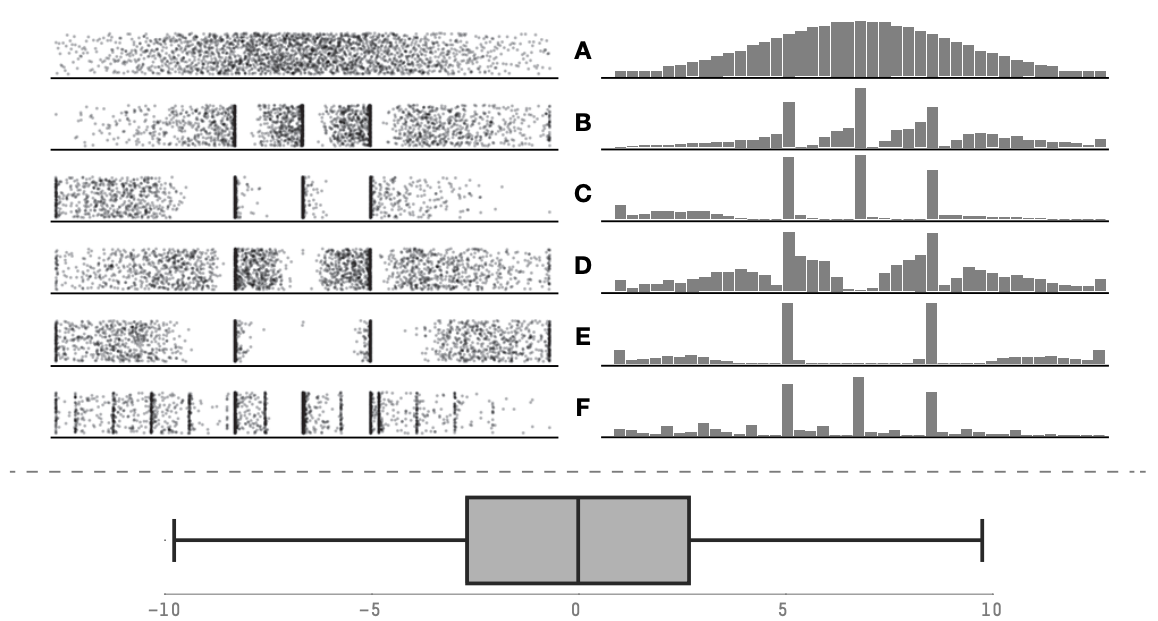
\includegraphics[width=0.5\textwidth]{histograms.png}}
	\caption{Cada letra es un conjunto de datos. Todos tienen los mismos valores de los cuartiles a pesar de ser conjuntos de datos muy diferentes.}
	\label{fig_sample}
\end{figure}

Otro tipo de gráfico muy común con variables numéricas es el de dispersión o scatter-plot, el cual permite ver si existe o no una relación entre dos variables numéricas (figura 3). 


\begin{figure}[htbp]
	\centerline{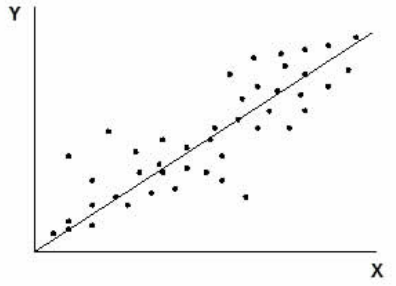
\includegraphics[width=0.3\textwidth]{scatterplot.png}}
	\caption{Diagrama de dispersión entre dos variables.}
	\label{fig_sample}
\end{figure}

\bigskip
\bigskip

\newpage

Generalmente a las variables numéricas se les toman medidas de tendencia y dispersión, de las más comunes son la media o el promedio y la desviación estándar (SD), respectivamente. Estas medidas son muy útiles pero se recomienda respaldarlas con gráficos. Por ejemplo, en la figura 4 se observan tres conjuntos de datos muy diferentes que producen la misma media, la misma desviación estándar e incluso la misma correlación. 

\begin{figure}[htbp]
	\centerline{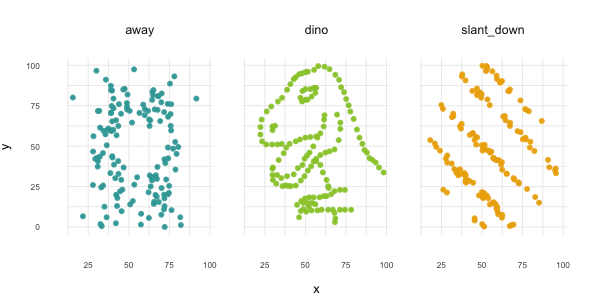
\includegraphics[width=0.5\textwidth]{datasaurus.png}}
	\caption{Datasaurus (media x=54.26, media y=47.83, SD x=16.76, SD y=26.93, correlación de Pearson=-0.06).}
	\label{fig_sample}
\end{figure}


\subsection{Gráficos con variables categóricas}

Otro tipo de variables con las que comúnmente trabajamos son las categóricas, que indican la presencia o ausencia de un atributo, o son indicadores de pertenencia a un grupo u otro. Para este tipo de variables sólo se pueden hacer conteos, por lo que se recomienden gráficos que coloquen el número de observaciones hechas para cada categoría. El gráfico de barras (figura 5) es de los más comunes.

\begin{figure}[htbp]
	\centerline{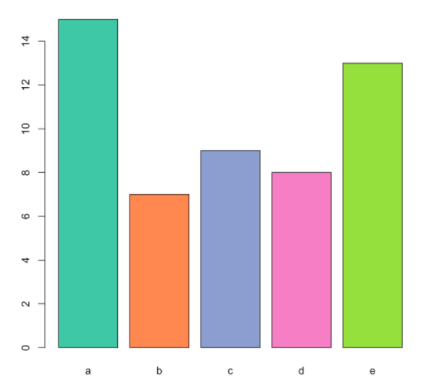
\includegraphics[width=0.3\textwidth]{barplot.png}}
	\caption{Gráfico de barras, conteos para cada categoría a, b, c, d o e.}
	\label{fig_sample}
\end{figure}

Existen otros tipos de variables como las de localización o temporales, así como muchas variaciones de gráficos e infinidad de representaciones visuales. Sin lugar a duda, la exploración de datos es uno de los aspectos más importantes e interesantes en los proyectos de ciencia de datos, pues está lleno de sorpresas, permite desarrollar creatividad, y reta a los científicos a expresar información de manera visual, sintetizada y que ayude a tomar decisiones en los siguientes pasos del proceso de investigación. 

% lleno de creatividad que puede generar muchos \textit{insights} muy útiles. 

\bigskip
\bigskip

\subsection*{Referencias:}

\begin{itemize}

\item Seminario de Métodos Analíticos de la Empresa, Taller de visualización. 

\item Matejka, J., \& Fitzmaurice, G. (2017, May). \textit{Same stats, different graphs: generating datasets with varied appearance and identical statistics through simulated annealing.} In Proceedings of the 2017 CHI Conference on Human Factors in Computing Systems (pp. 1290-1294).

\item Materia de Fundamentos en Estadística con Remuestreo, impartida por Teresa Ortiz \url{https://tereom.github.io/fundamentos/}

\item Materia de Introducción a la Ciencia de Datos, impartida por Liliana Millán.

\item \url{https://www.data-to-viz.com/}

\item \url{https://www.r-graph-gallery.com/}


\end{itemize}
	
% Elemen daftar pustaka yang disimpan dalam file Proposal.bib

\end{document}
